\documentclass[11pt,letterpaper]{article}

\usepackage[letterpaper,top=0.75in,bottom=0.85in,left=0.7in,right=0.7in]{geometry}
\usepackage{graphicx}
\usepackage{amsmath}
\usepackage{xcolor}
\usepackage{listings}
\usepackage{booktabs}
\usepackage{hyperref}
\usepackage{caption}
\usepackage{float}

\hypersetup{
    colorlinks=true,
    linkcolor=blue!60!black,
    urlcolor=blue!60!black,
}

% -----------------------------------------------------------------------------
% VHDL listing style
% -----------------------------------------------------------------------------
\definecolor{codebg}{RGB}{248,248,248}
\definecolor{codekw}{RGB}{0,0,180}
\definecolor{codecmt}{RGB}{0,120,0}
\definecolor{codestr}{RGB}{170,55,20}
\definecolor{codenum}{RGB}{120,120,120}

\lstdefinelanguage{VHDL2008}[]{VHDL}{
    morekeywords={
        library,use,entity,architecture,component,port,map,signal,variable,
        constant,begin,end,process,procedure,function,is,in,out,inout,
        std_logic,std_logic_vector,integer,unsigned,signed,to_integer,
        to_unsigned,to_signed,std,textio,ieee,numeric_std,std_logic_1164,
        rising_edge,falling_edge,wait,until,for,loop,if,then,else,elsif,others,
        severity,note,error,failure,warning,report,after,downto,upto,of,all,
        work,generic,case,when
    }
}

\lstset{
    language=VHDL2008,
    basicstyle=\ttfamily\small,
    keywordstyle=\color{codekw}\bfseries,
    commentstyle=\color{codecmt}\itshape,
    stringstyle=\color{codestr},
    numbers=left,
    numberstyle=\tiny\color{codenum},
    stepnumber=1,
    numbersep=6pt,
    backgroundcolor=\color{codebg},
    frame=single,
    rulecolor=\color{black!30},
    tabsize=4,
    showstringspaces=false,
    breaklines=true,
    breakatwhitespace=false,
    breakindent=0pt,
    postbreak=\mbox{\textcolor{red}{$\hookrightarrow$}\space},
    captionpos=b,
    aboveskip=8pt,
    belowskip=8pt,
    xleftmargin=8pt,
    xrightmargin=2pt,
    columns=fullflexible,
    keepspaces=true,
}

\lstdefinestyle{tcl}{
    language=tcl,
    morekeywords={set,puts,if,else,foreach,catch,source,create_ip,set_property,
                  get_ips,get_files,get_filesets,add_files,remove_files,
                  generate_target,export_ip_user_files,update_compile_order,
                  list_property,get_property,format,file,normalize,tail,
                  llength,lsort,info,exists,env,dirname,current_project,
                  ipx,save_core,write_hw_platform,launch_runs,wait_on_run},
    keywordstyle=\color{codekw}\bfseries,
}

% -----------------------------------------------------------------------------
% Title block
% -----------------------------------------------------------------------------
\title{\textbf{ECEC 661 -- Quiz 2 Submission}\\
       \large Add Constant $-1$ Custom AXI4-Lite IP}
\author{Gary Pham \texttt{(gp492)}}
\date{\today}

\begin{document}
\maketitle

% =============================================================================
\section{Problem Statement}
% =============================================================================

Create a custom AXI4-Lite IP using the Vivado IP-Catalog
\textbf{Adder/Subtractor} (\texttt{c\_addsub}). Configure the IP with a
\textbf{constant input} of $-1$. The data is 32-bit \emph{signed} and
clock-enable (CE) is \emph{disabled}. The user logic effectively computes:
\[
    z \;=\; x \;+\; (-1) \;=\; x - 1, \qquad x,z \in \text{signed 32-bit}.
\]

\begin{itemize}
    \item \textbf{Input} \texttt{x} : \texttt{std\_logic\_vector(31 downto 0)}
    \item \textbf{Output} \texttt{z} : \texttt{std\_logic\_vector(31 downto 0)}
    \item \textbf{Behaviour}: \texttt{z} is the combinational signed sum
          of \texttt{x} and the internal constant $-1$ (latency $= 0$,
          no clock).
\end{itemize}

The deliverables, per the hand-out, are: (1) a user-logic project with
simulation verifying the add-$(-1)$ logic; (2) the user logic packaged as
an AXI4-Lite IP; (3) a test-bench project with the custom IP attached to
the Zynq processor, generating the bitstream and exporting the
\texttt{.xsa} file. The Vitis test-app result is \emph{not} part of the
graded deliverables but is included at the end of this report for
completeness.

% =============================================================================
\section{IP Catalog Configuration}
% =============================================================================

The custom block \texttt{c\_addsub\_0} is generated from the Vivado IP
Catalog with the parameters listed in Table~\ref{tab:ipconfig}. The
\textbf{Constant Input} on port~B is the key knob: it removes B from the
external port list of the IP, leaving only \texttt{A[31:0]} and
\texttt{S[31:0]}.

\begin{table}[H]
    \centering
    \caption{\texttt{c\_addsub\_0} customisation parameters.}
    \label{tab:ipconfig}
    \begin{tabular}{ll}
        \toprule
        \textbf{Setting} & \textbf{Value} \\
        \midrule
        Implementation                & Fabric                                   \\
        Add Mode                      & Add ($S = A + B$)                        \\
        Port A Type / Width           & Signed / $32$                             \\
        Port B Type / Width           & Signed / $32$                             \\
        Port B \textbf{Constant Input}& enabled                                  \\
        Port B Constant Value (Bin)   & \texttt{1111\,1111\,1111\,1111\,1111\,1111\,1111\,1111} ($= -1$) \\
        Output Width                  & $32$                                     \\
        Latency Configuration         & Manual                                   \\
        Latency                       & $0$ (combinational)                      \\
        Clock Enable (CE)             & disabled                                 \\
        VLNV                          & \texttt{xilinx.com:ip:c\_addsub:12.0}    \\
        \bottomrule
    \end{tabular}
\end{table}

The equivalent Tcl automation from \texttt{scripts/setup.tcl} is:

\begin{lstlisting}[style=tcl,caption={Key IP-generation excerpt from
                   \texttt{setup.tcl}}]
create_ip -name c_addsub -vendor xilinx.com -library ip -version 12.0 \
          -module_name c_addsub_0

set_property -dict [list                                              \
    CONFIG.Implementation  {Fabric}                                   \
    CONFIG.A_Type          {Signed}                                   \
    CONFIG.B_Type          {Signed}                                   \
    CONFIG.A_Width         {32}                                       \
    CONFIG.B_Width         {32}                                       \
    CONFIG.Out_Width       {32}                                       \
    CONFIG.Add_Mode        {Add}                                      \
    CONFIG.B_Constant      {true}                                     \
    CONFIG.B_Value         {11111111111111111111111111111111}         \
    CONFIG.Latency         {0}                                        \
    CONFIG.CE              {false}                                    \
    CONFIG.SCLR            {false}                                    \
] [get_ips c_addsub_0]

generate_target {synthesis simulation} [get_ips c_addsub_0]
\end{lstlisting}

% =============================================================================
\section{User Logic HDL Code}
% =============================================================================

\texttt{user\_logic.vhd} is the deliverable user-logic file. It is a thin
wrapper that instantiates the IP-Catalog block and exposes the two ports
shown on the hand-out's IP-symbol diagram (\texttt{x[31:0]} input,
\texttt{z[31:0]} output).

\begin{lstlisting}[caption={user\_logic.vhd},label={lst:userlogic}]
library ieee;
use ieee.std_logic_1164.all;

entity user_logic is
    port (
        x : in  std_logic_vector(31 downto 0);
        z : out std_logic_vector(31 downto 0)
    );
end entity user_logic;

architecture rtl of user_logic is

    -- Vivado IP-Catalog Adder/Subtractor v12.0 (black box; elaborated from XCI).
    -- With Latency = 0 and B configured as a constant input, the only ports
    -- the IP exposes are A (signed input) and S (signed sum).  No CLK, no CE,
    -- no SCLR, no B port.
    component c_addsub_0
        port (
            A : in  std_logic_vector(31 downto 0);
            S : out std_logic_vector(31 downto 0)
        );
    end component;

begin

    U_ADDSUB : c_addsub_0
        port map (
            A => x,
            S => z
        );

end architecture rtl;
\end{lstlisting}

% =============================================================================
\section{S\_AXI Slave -- Component Instantiation and Port Map}
% =============================================================================

The hand-out asks specifically for the ``\texttt{S\_AXI} code where
component instantiation and port map'' is shown. The full AXI4-Lite slave
(\texttt{add\_const\_axi\_v1\_0\_S00\_AXI.vhd}) is the standard Xilinx
template; the code excerpt below is the section that wires
\texttt{user\_logic} into the AXI register file.

\begin{table}[H]
    \centering
    \caption{Software-visible register map exposed by the slave.}
    \label{tab:regmap}
    \begin{tabular}{lllp{8cm}}
        \toprule
        \textbf{Offset} & \textbf{Name} & \textbf{Access} & \textbf{Description} \\
        \midrule
        \texttt{0x00} & \texttt{X\_IN}  & R/W & 32-bit signed value driven into \texttt{user\_logic.x}. Reads return the last value written. \\
        \texttt{0x04} & \texttt{Z\_OUT} & R   & 32-bit signed result $z = x - 1$ from \texttt{user\_logic.z}. Writes ignored. \\
        \texttt{0x08} & --              & R/W & Reserved (returns $0$; writes ignored). \\
        \texttt{0x0C} & --              & R/W & Reserved (returns $0$; writes ignored). \\
        \bottomrule
    \end{tabular}
\end{table}

\begin{lstlisting}[caption={\texttt{add\_const\_axi\_v1\_0\_S00\_AXI.vhd} --
                   user\_logic component declaration, instantiation, and
                   read mux},label={lst:slv}]
-- Software-visible register: X_IN (slv_reg0).
signal slv_reg0 : std_logic_vector(31 downto 0);

-- Combinational result from the user logic (z = x - 1).
signal core_z  : std_logic_vector(31 downto 0);

signal reg_data_out : std_logic_vector(31 downto 0);

-- User-logic component declaration (deliverable: this is the "component
-- instantiation and port map" the quiz asks for).
component user_logic
    port (
        x : in  std_logic_vector(31 downto 0);
        z : out std_logic_vector(31 downto 0)
    );
end component;

begin

----------------------------------------------------------------------------
-- User-logic instantiation
--   x <- slv_reg0   (32-bit signed value written by software)
--   z -> core_z     (= x + (-1) from c_addsub_0; routed into the read mux)
----------------------------------------------------------------------------
U_LOGIC : user_logic
    port map (
        x => slv_reg0,
        z => core_z
    );

----------------------------------------------------------------------------
-- Register writes  (only X_IN is writable)
----------------------------------------------------------------------------
p_reg_write : process (S_AXI_ACLK)
    variable loc_addr : std_logic_vector(OPT_MEM_ADDR_BITS downto 0);
begin
    if rising_edge(S_AXI_ACLK) then
        if S_AXI_ARESETN = '0' then
            slv_reg0 <= (others => '0');
        else
            if slv_reg_wren = '1' then
                loc_addr := axi_awaddr(ADDR_LSB + OPT_MEM_ADDR_BITS
                                       downto ADDR_LSB);
                case loc_addr is
                    when "00" =>
                        for b in 0 to (C_S_AXI_DATA_WIDTH/8) - 1 loop
                            if S_AXI_WSTRB(b) = '1' then
                                slv_reg0(b*8 + 7 downto b*8) <=
                                    S_AXI_WDATA(b*8 + 7 downto b*8);
                            end if;
                        end loop;
                    when others =>
                        null;  -- 0x04 (Z_OUT) is read-only
                end case;
            end if;
        end if;
    end if;
end process p_reg_write;

----------------------------------------------------------------------------
-- Read mux:  0x00 -> X_IN readback,  0x04 -> Z_OUT (= x - 1)
----------------------------------------------------------------------------
p_read_mux : process (axi_araddr, slv_reg0, core_z)
    variable loc_addr : std_logic_vector(OPT_MEM_ADDR_BITS downto 0);
begin
    loc_addr := axi_araddr(ADDR_LSB + OPT_MEM_ADDR_BITS downto ADDR_LSB);
    case loc_addr is
        when "00" =>
            reg_data_out <= slv_reg0;       -- X_IN readback
        when "01" =>
            reg_data_out <= core_z;         -- Z_OUT = x - 1
        when others =>
            reg_data_out <= (others => '0');
    end case;
end process p_read_mux;
\end{lstlisting}

% =============================================================================
\section{Self-Checking Testbench}
% =============================================================================

\texttt{tb\_user\_logic.vhd} drives the DUT through \textbf{11 self-checks}
that exactly reproduce the reference run printed on the quiz hand-out
(\texttt{x = -5, -4, \ldots, 3} $\Rightarrow$ \texttt{z = x - 1}) and adds
two signed-boundary checks at \texttt{INT32\_MAX} and \texttt{INT32\_MIN}
to confirm the IP wraps modulo $2^{32}$ as a signed 32-bit adder must.

\begin{lstlisting}[caption={tb\_user\_logic.vhd -- excerpt of the
                   self-checking stimulus and check procedure},label={lst:tb}]
-- Quiz reference run, in order.
constant X_REF : int_vec := (-5, -4, -3, -2, -1,  0,  1,  2,  3);
constant Z_REF : int_vec := (-6, -5, -4, -3, -2, -1,  0,  1,  2);

-- Sample z and compare against the expected signed sum.
procedure check_z (
    signal   z_sig    : in    std_logic_vector(31 downto 0);
    constant expected : in    integer;
    constant xv       : in    integer;
    signal   err_cnt  : inout integer;
    signal   chk_cnt  : inout integer
) is
    variable got : integer;
begin
    got     := to_integer(signed(z_sig));
    chk_cnt <= chk_cnt + 1;
    if got = expected then
        report "[PASS] x=" & integer'image(xv) &
               "  z=" & integer'image(got) severity note;
    else
        report "[FAIL] x=" & integer'image(xv) &
               "  got z=" & integer'image(got) &
               "  expected=" & integer'image(expected)
            severity error;
        err_cnt <= err_cnt + 1;
    end if;
end procedure check_z;

-- ... clock, DUT, p_clk omitted ...

p_stim : process
begin
    -- Reference run from the quiz hand-out.
    for i in X_REF'range loop
        x <= std_logic_vector(to_signed(X_REF(i), 32));
        wait until rising_edge(ck);
        wait for 1 ns;
        check_z(z, Z_REF(i), X_REF(i), errors, checks);
    end loop;

    -- Signed boundary cases.
    x <= std_logic_vector(to_signed( 2147483647, 32));
    wait until rising_edge(ck); wait for 1 ns;
    check_z(z,  2147483646,  2147483647, errors, checks);

    x <= std_logic_vector(to_signed(-2147483648, 32));
    wait until rising_edge(ck); wait for 1 ns;
    check_z(z,  2147483647, -2147483648, errors, checks); -- signed wrap
    wait;
end process p_stim;
\end{lstlisting}

% =============================================================================
\section{Simulation Results}
% =============================================================================

\subsection{Waveform}

Figure~\ref{fig:wave} shows the xsim behavioural simulation. The input
\texttt{x} (signed decimal) and the output \texttt{z} (signed decimal)
are displayed alongside the running \texttt{checks} counter. \texttt{z}
follows \texttt{x} exactly one combinational cycle later because the IP
has Latency $= 0$.

\begin{figure}[H]
    \centering
    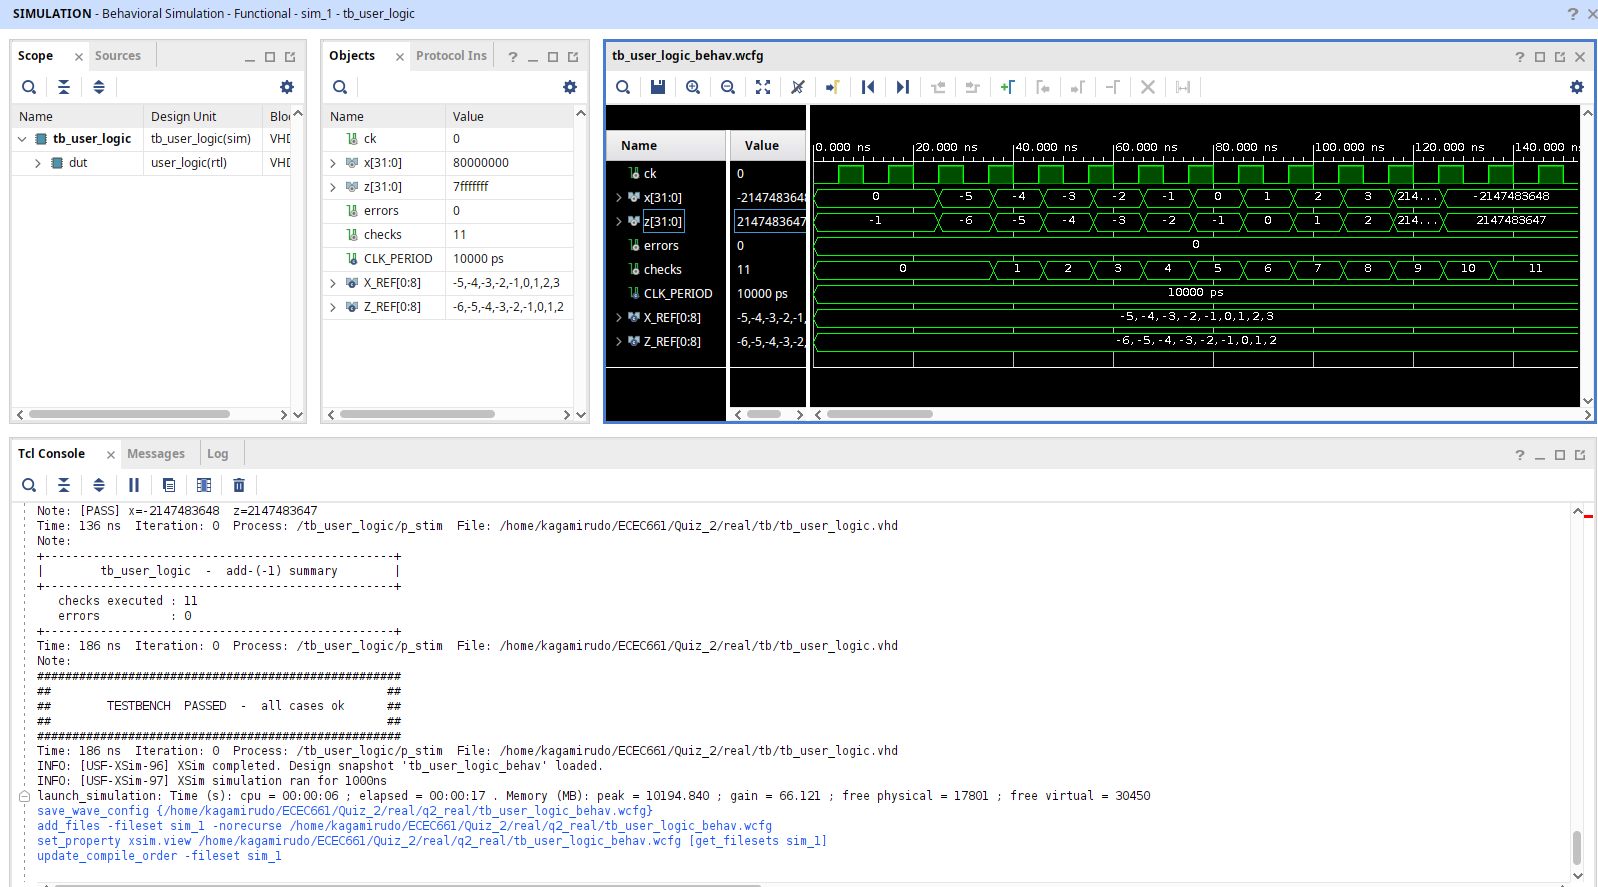
\includegraphics[width=\textwidth]{sim_result.png}
    \caption{Behavioural simulation of \texttt{tb\_user\_logic}. The
             input \texttt{x} walks the reference run
             $-5,\,-4,\,\dots,\,3$ and the boundary cases
             \texttt{INT32\_MAX} and \texttt{INT32\_MIN}. The output
             \texttt{z} consistently equals \texttt{x - 1} (with the
             expected signed wrap on \texttt{INT32\_MIN}).}
    \label{fig:wave}
\end{figure}

\subsection{Console output}

All 11 self-checks pass:

\begin{lstlisting}[language={},basicstyle=\ttfamily\small,
                    numbers=none,backgroundcolor=\color{codebg},
                    frame=single,breaklines=true,
                    xleftmargin=8pt,xrightmargin=2pt]
[PASS] x=-5  z=-6
[PASS] x=-4  z=-5
[PASS] x=-3  z=-4
[PASS] x=-2  z=-3
[PASS] x=-1  z=-2
[PASS] x=0   z=-1
[PASS] x=1   z=0
[PASS] x=2   z=1
[PASS] x=3   z=2
[PASS] x=2147483647   z=2147483646
[PASS] x=-2147483648  z=2147483647

+--------------------------------------------------+
|        tb_user_logic  -  add-(-1) summary        |
+--------------------------------------------------+
   checks executed : 11
   errors          : 0
+--------------------------------------------------+

####################################################
##                                                ##
##        TESTBENCH  PASSED  -  all cases ok      ##
##                                                ##
####################################################
\end{lstlisting}

% =============================================================================
\section{IP Packaging}
% =============================================================================

The user logic and AXI4-Lite slave are packaged together as a single
custom IP \texttt{add\_const\_axi v1.0} via
\textit{Tools $\rightarrow$ Create and Package New IP $\rightarrow$
Package your current project}, with the IP location set to
\texttt{ip\_repo/add\_const\_axi\_1.0}. The Tcl helper
\texttt{scripts/package.tcl} fills in the metadata fields and adds the
sub-core reference to the IP-Catalog adder so the packaged IP carries
\texttt{c\_addsub} along with it:

\begin{lstlisting}[style=tcl,caption={Excerpt of \texttt{package.tcl} --
                   identification, sub-core reference, clock parameters}]
set core [ipx::current_core]

set_property vendor       user                                          $core
set_property library      user                                          $core
set_property name         add_const_axi                                 $core
set_property version      1.0                                           $core
set_property display_name "Add Constant -1 AXI4-Lite Core"              $core
set_property taxonomy     /UserIP                                       $core

# Sub-core reference.  Adds c_addsub to BOTH file groups so the packaged IP
# pulls the IP-Catalog block in along with the wrapper.
foreach fg {xilinx_vhdlsynthesis xilinx_vhdlbehavioralsimulation} {
    set group [ipx::get_file_groups $fg -of_objects $core]
    if {$group ne ""} {
        ipx::add_subcore_reference xilinx.com:ip:c_addsub:12.0 $group
    }
}

# AXI clock parameters (FREQ_HZ, ASSOCIATED_BUSIF, ASSOCIATED_RESET) clear
# the usual 19-11770 and 19-7067 packager warnings.
set aclk [ipx::get_bus_interfaces s00_axi_aclk -of_objects $core]
ipx::add_bus_parameter FREQ_HZ          $aclk
ipx::add_bus_parameter ASSOCIATED_BUSIF $aclk
ipx::add_bus_parameter ASSOCIATED_RESET $aclk

ipx::save_core $core
\end{lstlisting}

After running \texttt{package.tcl} the IP Packager's
\textit{Review and Package} pane shows zero outstanding warnings, at
which point \textit{Re-Package IP} re-zips the core and closes the
packager project.

% =============================================================================
\section{Block Design and \texttt{.xsa} Export}
% =============================================================================

The packaged \texttt{add\_const\_axi} IP is added to the project's IP
repository, then dropped into a small Zynq block design alongside the
\texttt{ZYNQ7 Processing System} and an \texttt{AXI Interconnect}
(Figure~\ref{fig:bd}). \textit{Run Connection Automation} wires the
\texttt{FCLK\_CLK0} clock and \texttt{peripheral\_aresetn} reset to every
AXI block. The IP is mapped at base address
\texttt{0x4300\_0000}\footnote{Equivalent to \texttt{0x43C0\_0000} on
Cora Z7-07S.} with a $4\,\text{KB}$ aperture in the Address Editor.

\begin{figure}[H]
    \centering
    \includegraphics[width=\textwidth]{{diagram with xsa}.png}
    \caption{Block diagram of the test-bench project: Zynq~PS
             (\texttt{processing\_system7\_0}) drives the AXI Interconnect,
             which masters the custom \texttt{add\_const\_axi\_0} slave.
             \textit{Validate Design} returns clean; the same project
             produces the bitstream and is the source of the exported
             \texttt{add\_const.xsa}.}
    \label{fig:bd}
\end{figure}

After \textit{Validate Design} $\rightarrow$ \textit{Generate Output
Products} $\rightarrow$ \textit{Create HDL Wrapper}, synthesis,
implementation, and bitstream generation are run, and the
\texttt{.xsa} is exported through:

\begin{lstlisting}[style=tcl,caption={Bitstream and \texttt{.xsa} export}]
launch_runs synth_1 -jobs 4
wait_on_run synth_1
launch_runs impl_1 -to_step write_bitstream -jobs 4
wait_on_run impl_1

file mkdir xsa
write_hw_platform -fixed -include_bit -force \
    -file xsa/add_const.xsa
\end{lstlisting}

% =============================================================================
\section{Vitis Test Application (optional)}
% =============================================================================

The Vitis bare-metal test app (\texttt{sw/main.c}) is \emph{not} part of
the graded deliverables but is provided as confirmation that the
packaged IP exchanges data correctly with software through the AXI
register map. The app:

\begin{enumerate}
    \item Probes the IP at the published base address with a known
          marker (\texttt{0xA5A5A5A5}) to fail fast if the bus is wired
          incorrectly;
    \item Walks the same reference run as the testbench
          (\texttt{x = -5, \ldots, 3}) plus the signed boundary cases;
    \item Prints each result in a boxed ASCII table over UART.
\end{enumerate}

Figure~\ref{fig:vitis} shows the Vitis Serial Monitor capture: every
test vector returns the expected \texttt{z = x - 1}, including the
\texttt{INT32\_MIN} signed wrap (\texttt{0x8000\,0000} $\to$
\texttt{0x7FFF\,FFFF}).

\begin{figure}[H]
    \centering
    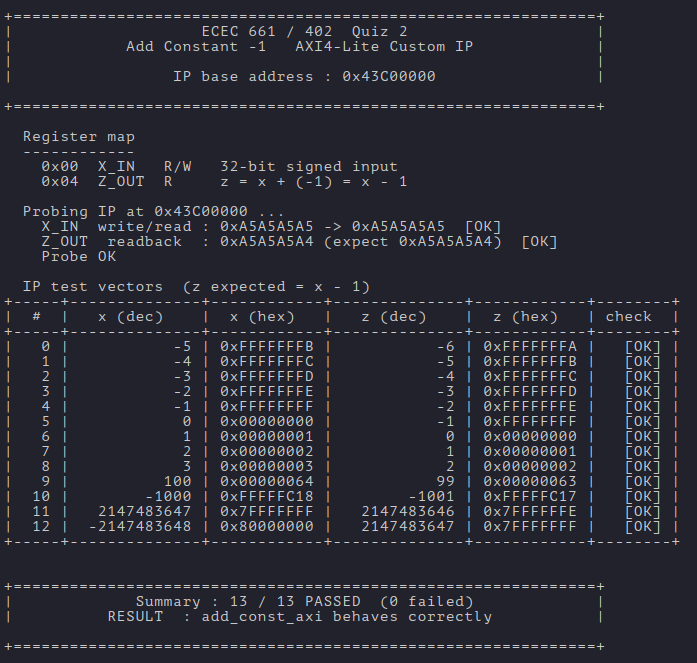
\includegraphics[width=\textwidth]{vitis_result.png}
    \caption{Vitis Serial Monitor output for \texttt{add\_const\_app}.
             The probe banner confirms AXI write/read works at base
             address \texttt{0x43C0\_0000}; the test table then prints
             13 vectors (the hand-out reference run plus 4 boundary
             cases), all marked \texttt{[OK]}, and the run finishes with
             \texttt{Summary : 13 / 13 PASSED}.}
    \label{fig:vitis}
\end{figure}

% =============================================================================
\section{Conclusion}
% =============================================================================

The custom \texttt{add\_const\_axi} IP behaves exactly as specified:

\begin{itemize}
    \item The IP-Catalog Adder/Subtractor is configured with a constant
          $B = -1$ on a 32-bit signed bus, latency $0$, no CE, so the
          user logic computes $z = x - 1$ combinationally.
    \item All 11 self-checks in \texttt{tb\_user\_logic.vhd} return
          \texttt{[PASS]} and the simulator finishes with the
          \textit{TESTBENCH PASSED} banner; the waveform in
          Figure~\ref{fig:wave} matches the reference run printed on
          the hand-out.
    \item Packaging into \texttt{user/user/add\_const\_axi/1.0} is clean
          (no \texttt{19-11888 / 19-896 / 19-11770 / 19-7067}
          warnings), with the \texttt{c\_addsub:12.0} sub-core reference
          attached to both VHDL Synthesis and VHDL Simulation file
          groups.
    \item The block design (Figure~\ref{fig:bd}) validates, the
          bitstream builds, and \texttt{add\_const.xsa} is exported
          successfully via \texttt{write\_hw\_platform}.
\end{itemize}

The optional Vitis bare-metal app (Figure~\ref{fig:vitis}) confirms the
packaged IP integrates with the PS through the AXI register map:
software writes \texttt{X\_IN}, reads \texttt{Z\_OUT}, and observes
$z = x - 1$ on every test vector.

\end{document}
